% cmnotes_test.tex

% comment/uncomment the following to test the various options

% proofs
%\PassOptionsToPackage{noproofs}{cmnotes}
%\PassOptionsToPackage{blankproofs}{cmnotes}

% solutions
%\PassOptionsToPackage{nosolutions}{cmnotes}
%\PassOptionsToPackage{blanksolutions}{cmnotes}

% answers
%\PassOptionsToPackage{noanswers}{cmnotes}
%\PassOptionsToPackage{blankanswers}{cmnotes}

% images
%\PassOptionsToPackage{blankimages}{cmnotes}
%\PassOptionsToPackage{blankallimages}{cmnotes}

% misc
%\PassOptionsToPackage{blanktext}{cmnotes}
%\PassOptionsToPackage{student}{cmnotes}

%----------------------------------------
\documentclass{article}
%----------------------------------------

\usepackage{cmnotes}
\usepackage{graphicx}
\usepackage{lipsum}

% document info
\title{Test Document for \texttt{cmnotes.sty}}
\author{D Evans \& D McConnell}
\date{Autumn 2017}

% layout
\setlength{\parindent}{0em}
\setlength{\parskip}{0.5em}
\usepackage[a4paper, margin=20mm]{geometry}

% theorem types
\usepackage{ntheorem}
\theoremstyle{break}
\theorembodyfont{\upshape}
\newcounter{theorem}
\newtheorem{theorem}{Theorem}
\newtheorem{definition}[theorem]{Definition}
\newtheorem{lemma}[theorem]{Lemma}
\newtheorem{example}[theorem]{Example}
\newtheorem{exercise}[theorem]{Exercise}
\newtheorem{quiz}[theorem]{Quiz}

% Set stretch factor for blank boxes and images
\setstretchfactor{2} 
\setscaleimages{1.5} 
% the latter should be called \setimagestretchfactor 
% it doesn't seem to work anymore!

% more cmnotes options
\textcolour{black}
\proofcolour{blue}
\answercolour{red}
\solutioncolour{purple}
\showcolour{ForestGreen}


%----------------------------------------
\begin{document}
\maketitle
\tableofcontents
\bigskip
\hrule
\begin{center}
This is a test document for the {\tt cmnotes.sty} package. The latest version can be found at
\par
\texttt{https://github.com/cardiffmaths/texmf/tex/latex/cmnotes}
\end{center}
\hrule

%----------------------------------------
\section{Theorems}

\begin{theorem}\label{thm:test}
This is the statement of the theorem.
\begin{proof}
This is a proof of the theorem.\par
Let's give it a few lines.\par
Like this one.
\end{proof}
\end{theorem}

The visibility of {\tt proof} environments is controlled by the following package options.

\bigskip
\begin{tabular}{ll}
\hline
{\tt proofs}		& print contents (default) \\
{\tt blankproofs}	& print blank box \\
{\tt noproofs}		& print nothing \\
\hline
\end{tabular}
\bigskip

%--------------------
\subsection{Examples}
The {\tt example} theorem type is defined in the preamble.

\begin{example}
The integral of $f(x)=x$ over the interval $[0,1]$ is
\[
\int_0^1 x\,dx = \left[\frac{x^2}{2}\right]_0^1 = \frac{1}{2}
\]
\end{example}

Examples can have {\tt solutions}.
\begin{example}
Find the integral of $f(x)=x$ over the interval $[0,1]$.
\begin{solution}
$f(x)$ is bounded over $[0,1]$ so 
\[
\int_0^1 x\,dx = \left[\frac{x^2}{2}\right]_0^1 = \frac{1}{2}
\]
\end{solution}
\end{example}

The visibility of {\tt solution} environments is controlled by the following package options.

\bigskip
\begin{tabular}{ll}
\hline
{\tt solutions}			& print contents (default) \\
{\tt blanksolutions}	& print blank box \\
{\tt nosolutions}		& print nothing \\
\hline
\end{tabular}
\bigskip

The same result be achieved using the {\tt blankbox} environment, but without the heading.
\begin{example}
Find the integral of $f(x)=x$ over the interval $[0,1]$.
\begin{blankbox}
$f(x)$ is bounded over $[0,1]$ so 
\[
\int_0^1 x\,dx = \left[\frac{x^2}{2}\right]_0^1 = \frac{1}{2}
\]
\end{blankbox}
\end{example}

The visibility of {\tt blankbox} environments is controlled by the following package options.

\bigskip
\begin{tabular}{ll}
\hline
{\tt noblanktext}		& print contents (default) \\
{\tt blanktext}			& print blank box \\
\hline
\end{tabular}
\bigskip

%--------------------
\subsection{Exercises and quizzes}
The {\tt exercise} and {\tt quiz} theorem types are defined the preamble.

\begin{exercise}\label{exe:test}
This is an exercise. 
\end{exercise}

\begin{quiz}\label{quiz:test}
This is a quiz. 
\end{quiz}

These serve as containers for various types of question (see below).

%----------------------------------------
\section{Question types (copied from \texttt{exam.cls})}
%----------------------------------------

\verb+\ans+ commands and {\tt answer} environments can be inserted anywhere. Their visibility is controlled by the following package options.

\bigskip
\begin{tabular}{ll}
\hline
{\tt answers}		& print contents (default) \\
{\tt blankanswers}	& print  blank box \\
{\tt noanswers}		& print nothing \\
\hline
\end{tabular}
\bigskip

Here is an answer (it might not be visible):
\begin{answer}
%But what is the question?
\lipsum[1]
\end{answer}

We can force answers to be included using \verb+\answerson ... \endanswerson+. The following answer will always be included.
\answerson
\begin{answer}
This is always included
\end{answer}
\endanswerson

We can force answers to be excluded using  \verb+\answersoff ... \endanswersoff+. The following answer will never be included.
\answersoff
\begin{answer}
This is never included
\end{answer}
\endanswersoff

%--------------------
\subsection{Questions, parts and subparts}

Here is an exercise containing a {\tt questions} environment, which itself contains a {\tt parts} environment. 
\begin{exercise}\label{exe:demo}
\begin{questions}
\question First question.
\begin{parts}
\part First part.
\ans{Answer to the first part.}
\part Second part.
\begin{subparts}
\subpart First subpart.
\ans{Answer to the first subpart.}
\subpart Second subpart.
\ans{Answer to the second subpart.}
\end{subparts}
\end{parts}
\question Second question.
\ans{Answer to the second question.}
\end{questions}
\end{exercise}


%--------------------
\subsection{Multiple choice and multiple answer questions}

The following quiz has two multiple choice questions (\texttt{choices}), two multiple answer questions (\texttt{checkboxes}) questions, and a free-text question (default).

\begin{quiz}
\begin{questions} 

% true or false (implemented using multiple choice)
\question Necessity is the mother of invention.
\begin{choices}
\correctchoice True 		
\choice False		
\end{choices}

% multiple choice question
\question In what year did Columbus first cross the Atlantic?
\begin{choices}
\choice 1490 %\begin{response} Sorry, better luck next time.\end{response}
\choice 1491 %\begin{response} Sorry, better luck next time.\end{response}
\correctchoice   1492 %\begin{response} Correct, well done.\end{response} 
\choice 1493 %\begin{response} Sorry, better luck next time.\end{response}
\end{choices}
\begin{answer}
In 1492, Columbus sailed the ocean blue.
\end{answer}

% multiple answer question 
\question
\label{qu:series}
Which of the following series converge?
\begin{checkboxes}
\choice $\sum_{n=1}^{\infty}\frac{1}{n}$
\correctchoice $\sum_{n=1}^{\infty}\frac{1}{n^2}$
\correctchoice $\sum_{n=1}^{\infty}\frac{1}{n^4}$
\end{checkboxes}
\begin{answer}
\begin{itemize}
\item $\sum_{n=1}^{\infty}\frac{1}{n}$ diverges (this is the harmonic series). 
\item $\sum_{n=1}^{\infty}\frac{1}{n^2} = \pi^2/6$.
\item $\sum_{n=1}^{\infty}\frac{1}{n^4} = \pi^4/90$.
\end{itemize}
\end{answer}

% free text
\question 
Write a short essay on a topic of your choice.  
\begin{answer}
Anything sensible will do.
\end{answer}

\end{questions}
\end{quiz}


%----------------------------------------
\section{Blanks}
%----------------------------------------
Here is a {\tt blankbox} command. This is controlled by the {\tt blanktext} option. There is an issue with indentation here.
\begin{blankbox}
Can you see me?\\ Another line here.\\ And another.
\end{blankbox}

Then we move on.

%----------------------------------------
\section{Figures}
%----------------------------------------

\begin{example}
The upper half plane $H_+$ defined by
\[
H_+:= \left\{ z \in \mathbb{C}: \Im (z) > 0\right\}
\]
is an open set.
\end{example}

\begin{solution}
We shall show that for any $z \in H_+$, we can find an open disc centred at $z$ that is entirely contained in $H_+$.
\begin{center}
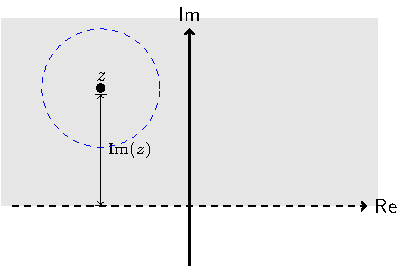
\includegraphics[scale=1]{upperhalf_full.pdf}
\end{center}
There we are.
\end{solution}

An incomplete image can be printed in the student version, and a complete imaage in the full version.
\begin{example}
\label{e:upperhalfplane2}
The upper half plane $H_+$ defined by
\[
H_+:= \left\{z \in \mathbb{C}: \Im (z) > 0 \right\}
\]
is an open set.
\end{example}
\begin{solution}
\begin{center}
\altgraphics[scale=1]{upperhalf_full}{upperhalf_partial}
\end{center}
We have shown that for every $z \in H_+$, there is an open disc centred at $z$ that is entirely contained in $H_+$.  Observe that the picture is now smaller.
\end{solution}

It is not snecessary to use the example--solution format to achieve this, as Example~\ref{e:upperhalfplane3} shows.
\begin{example}
\label{e:upperhalfplane3}
The upper half plane $H_+$ defined by
\[
H_+:= \left\{z \in \mathbb{C}: \Im (z) > 0 \right\}
\]
is an open set.
\blankson
\begin{center}
\altgraphics[scale=1]{upperhalf_full}{upperhalf_partial}
\end{center}
We have shown that for every $z \in H_+$, there is an open disc centred at $z$ that is entirely contained in $H_+$.  Observe that the picture is now smaller.
\blanksoff
\end{example}

Then we move on. 

Still it might be better to use a {\tt blankbox} environment instead of the \verb+\blankson+ and \verb+\blanksoff+ commands, so that students are clear that there is something for them to complete here. It also makes it possible to change the font colour to make it clear what appears in the full version and not in the student version. For example,

\begin{example}
The upper half plane $H_+$ defined by
\[
H_+:= \left\{z \in \mathbb{C}: \Im (z) > 0 \right\}
\]
is an open set.
\begin{blankbox}
\begin{center}
\altgraphics[scale=1]{upperhalf_full}{upperhalf_partial}
\end{center}
We have shown that for every $z \in H_+$, there is an open disc centred at $z$ that is entirely contained in $H_+$.  Observe that the picture is now smaller.
\end{blankbox}
\end{example}
Then we move on.
%\begin{solution}
%\lipsum[1]
%\blankson
%\lipsum[2]
%\begin{center}
%\begin{tikzpicture}
%\draw (0,0) circle (2);
%\end{tikzpicture}
%\end{center}
%\blanksoff
%\lipsum[3]
%\end{solution}
%For completeness, we include a picture of a black square:
%\begin{center}
%\begin{tikzpicture}
%\draw[fill] (-3,-3) rectangle  (3,3);
%\end{tikzpicture}
%\end{center}
%

%========================================
\end{document}
%========================================


